\documentclass[]{book}
\usepackage{lmodern}
\usepackage{amssymb,amsmath}
\usepackage{ifxetex,ifluatex}
\usepackage{fixltx2e} % provides \textsubscript
\ifnum 0\ifxetex 1\fi\ifluatex 1\fi=0 % if pdftex
  \usepackage[T1]{fontenc}
  \usepackage[utf8]{inputenc}
\else % if luatex or xelatex
  \ifxetex
    \usepackage{mathspec}
  \else
    \usepackage{fontspec}
  \fi
  \defaultfontfeatures{Ligatures=TeX,Scale=MatchLowercase}
\fi
% use upquote if available, for straight quotes in verbatim environments
\IfFileExists{upquote.sty}{\usepackage{upquote}}{}
% use microtype if available
\IfFileExists{microtype.sty}{%
\usepackage{microtype}
\UseMicrotypeSet[protrusion]{basicmath} % disable protrusion for tt fonts
}{}
\usepackage[margin=1in]{geometry}
\usepackage{hyperref}
\hypersetup{unicode=true,
            pdftitle={R notes for S\&DS 220},
            pdfborder={0 0 0},
            breaklinks=true}
\urlstyle{same}  % don't use monospace font for urls
\usepackage{natbib}
\bibliographystyle{apalike}
\usepackage{color}
\usepackage{fancyvrb}
\newcommand{\VerbBar}{|}
\newcommand{\VERB}{\Verb[commandchars=\\\{\}]}
\DefineVerbatimEnvironment{Highlighting}{Verbatim}{commandchars=\\\{\}}
% Add ',fontsize=\small' for more characters per line
\usepackage{framed}
\definecolor{shadecolor}{RGB}{248,248,248}
\newenvironment{Shaded}{\begin{snugshade}}{\end{snugshade}}
\newcommand{\AlertTok}[1]{\textcolor[rgb]{0.94,0.16,0.16}{#1}}
\newcommand{\AnnotationTok}[1]{\textcolor[rgb]{0.56,0.35,0.01}{\textbf{\textit{#1}}}}
\newcommand{\AttributeTok}[1]{\textcolor[rgb]{0.77,0.63,0.00}{#1}}
\newcommand{\BaseNTok}[1]{\textcolor[rgb]{0.00,0.00,0.81}{#1}}
\newcommand{\BuiltInTok}[1]{#1}
\newcommand{\CharTok}[1]{\textcolor[rgb]{0.31,0.60,0.02}{#1}}
\newcommand{\CommentTok}[1]{\textcolor[rgb]{0.56,0.35,0.01}{\textit{#1}}}
\newcommand{\CommentVarTok}[1]{\textcolor[rgb]{0.56,0.35,0.01}{\textbf{\textit{#1}}}}
\newcommand{\ConstantTok}[1]{\textcolor[rgb]{0.00,0.00,0.00}{#1}}
\newcommand{\ControlFlowTok}[1]{\textcolor[rgb]{0.13,0.29,0.53}{\textbf{#1}}}
\newcommand{\DataTypeTok}[1]{\textcolor[rgb]{0.13,0.29,0.53}{#1}}
\newcommand{\DecValTok}[1]{\textcolor[rgb]{0.00,0.00,0.81}{#1}}
\newcommand{\DocumentationTok}[1]{\textcolor[rgb]{0.56,0.35,0.01}{\textbf{\textit{#1}}}}
\newcommand{\ErrorTok}[1]{\textcolor[rgb]{0.64,0.00,0.00}{\textbf{#1}}}
\newcommand{\ExtensionTok}[1]{#1}
\newcommand{\FloatTok}[1]{\textcolor[rgb]{0.00,0.00,0.81}{#1}}
\newcommand{\FunctionTok}[1]{\textcolor[rgb]{0.00,0.00,0.00}{#1}}
\newcommand{\ImportTok}[1]{#1}
\newcommand{\InformationTok}[1]{\textcolor[rgb]{0.56,0.35,0.01}{\textbf{\textit{#1}}}}
\newcommand{\KeywordTok}[1]{\textcolor[rgb]{0.13,0.29,0.53}{\textbf{#1}}}
\newcommand{\NormalTok}[1]{#1}
\newcommand{\OperatorTok}[1]{\textcolor[rgb]{0.81,0.36,0.00}{\textbf{#1}}}
\newcommand{\OtherTok}[1]{\textcolor[rgb]{0.56,0.35,0.01}{#1}}
\newcommand{\PreprocessorTok}[1]{\textcolor[rgb]{0.56,0.35,0.01}{\textit{#1}}}
\newcommand{\RegionMarkerTok}[1]{#1}
\newcommand{\SpecialCharTok}[1]{\textcolor[rgb]{0.00,0.00,0.00}{#1}}
\newcommand{\SpecialStringTok}[1]{\textcolor[rgb]{0.31,0.60,0.02}{#1}}
\newcommand{\StringTok}[1]{\textcolor[rgb]{0.31,0.60,0.02}{#1}}
\newcommand{\VariableTok}[1]{\textcolor[rgb]{0.00,0.00,0.00}{#1}}
\newcommand{\VerbatimStringTok}[1]{\textcolor[rgb]{0.31,0.60,0.02}{#1}}
\newcommand{\WarningTok}[1]{\textcolor[rgb]{0.56,0.35,0.01}{\textbf{\textit{#1}}}}
\usepackage{longtable,booktabs}
\usepackage{graphicx,grffile}
\makeatletter
\def\maxwidth{\ifdim\Gin@nat@width>\linewidth\linewidth\else\Gin@nat@width\fi}
\def\maxheight{\ifdim\Gin@nat@height>\textheight\textheight\else\Gin@nat@height\fi}
\makeatother
% Scale images if necessary, so that they will not overflow the page
% margins by default, and it is still possible to overwrite the defaults
% using explicit options in \includegraphics[width, height, ...]{}
\setkeys{Gin}{width=\maxwidth,height=\maxheight,keepaspectratio}
\IfFileExists{parskip.sty}{%
\usepackage{parskip}
}{% else
\setlength{\parindent}{0pt}
\setlength{\parskip}{6pt plus 2pt minus 1pt}
}
\setlength{\emergencystretch}{3em}  % prevent overfull lines
\providecommand{\tightlist}{%
  \setlength{\itemsep}{0pt}\setlength{\parskip}{0pt}}
\setcounter{secnumdepth}{5}
% Redefines (sub)paragraphs to behave more like sections
\ifx\paragraph\undefined\else
\let\oldparagraph\paragraph
\renewcommand{\paragraph}[1]{\oldparagraph{#1}\mbox{}}
\fi
\ifx\subparagraph\undefined\else
\let\oldsubparagraph\subparagraph
\renewcommand{\subparagraph}[1]{\oldsubparagraph{#1}\mbox{}}
\fi

%%% Use protect on footnotes to avoid problems with footnotes in titles
\let\rmarkdownfootnote\footnote%
\def\footnote{\protect\rmarkdownfootnote}

%%% Change title format to be more compact
\usepackage{titling}

% Create subtitle command for use in maketitle
\newcommand{\subtitle}[1]{
  \posttitle{
    \begin{center}\large#1\end{center}
    }
}

\setlength{\droptitle}{-2em}
  \title{R notes for S\&DS 220}
  \pretitle{\vspace{\droptitle}\centering\huge}
  \posttitle{\par}
  \author{}
  \preauthor{}\postauthor{}
  \predate{\centering\large\emph}
  \postdate{\par}
  \date{2018-03-27}

\usepackage{booktabs}

\usepackage{amsthm}
\newtheorem{theorem}{Theorem}[chapter]
\newtheorem{lemma}{Lemma}[chapter]
\theoremstyle{definition}
\newtheorem{definition}{Definition}[chapter]
\newtheorem{corollary}{Corollary}[chapter]
\newtheorem{proposition}{Proposition}[chapter]
\theoremstyle{definition}
\newtheorem{example}{Example}[chapter]
\theoremstyle{definition}
\newtheorem{exercise}{Exercise}[chapter]
\theoremstyle{remark}
\newtheorem*{remark}{Remark}
\newtheorem*{solution}{Solution}
\begin{document}
\maketitle

{
\setcounter{tocdepth}{1}
\tableofcontents
}
\hypertarget{about}{%
\chapter*{About}\label{about}}
\addcontentsline{toc}{chapter}{About}

These notes organize and summarize the R material you need to know for
S\&DS 220.

\hypertarget{basics}{%
\chapter{Basics}\label{basics}}

\hypertarget{setting-up}{%
\section{Setting up}\label{setting-up}}

R is a programming language that's popular for data manipulation. An
up-to-date R interpreter can be downloaded from
\href{https://www.r-project.org/}{r-project.org}. After downloading and
installing the interpreter, you'll also want to download and install
\href{https://www.rstudio.com/}{RStudio} which provides a helpful visual
interface for you to work with the interpreter.

\hypertarget{language-fundamentals}{%
\section{Language fundamentals}\label{language-fundamentals}}

Open RStudio, and find the box labeled \textbf{Console}. There should be
a blinking \texttt{\textbar{}} to the right of the
\texttt{\textgreater{}} at the bottom of the box; if there isn't, then
click to the right of \texttt{\textgreater{}}. Now type \texttt{1+2} and
hit enter. The R interpreter reads your message and responds with
\texttt{{[}1{]}\ 3}. Ignore the \texttt{{[}1{]}} for now; the R
interpreter acted like a calculator and told us that 1+2 is 3. Next type
\texttt{a\ \textless{}-\ 1+2} and hit enter. This time the result of the
calculation \texttt{1+2} is stored as an object called \texttt{a}. Type
\texttt{a} and hit enter to see its value.

Let's see one more quick example. Type \texttt{1:100} and hit enter.
This is a convenient way to create a vector comprising the integers from
1 to 100.

\begin{center}\rule{0.5\linewidth}{\linethickness}\end{center}

\textbf{Exercise:} Try the command \texttt{rep(1,\ 100)}. What does it
do? Looking at the interpreter's response to this command and to
\texttt{1:100}, figure out what the \texttt{{[}1{]}} means.

\begin{center}\rule{0.5\linewidth}{\linethickness}\end{center}

\textbf{Exercise:} Make a guess at what R's response to the following
commands will be. Then try them and explain what you think they're
doing. (If you have no idea what to guess, just try it and see what
happens.)

\begin{itemize}
\tightlist
\item
  \texttt{(1:5)\^{}2}
\item
  \texttt{sum(1:5)}
\item
  \texttt{sum(rep(1,\ 5))}
\item
  \texttt{mean(1:5)}
\item
  \texttt{prod(1:5)}
\item
  \texttt{max(1:5)\ -\ min(1:5)}
\item
  \texttt{1:4\ +\ 3:6}
\item
  \texttt{2\ *\ (1:4)}
\item
  \texttt{1:4\ *\ 3:6}
\item
  \texttt{log(1:4)}
\item
  \texttt{log10(1:4)}
\item
  \texttt{sqrt(1:4)}
\item
  \texttt{c(1,\ 3,\ 5)}
\item
  \texttt{c(1:4,\ 1,\ 3,\ 5)}
\item
  \texttt{v\ \textless{}-\ c(c(1,\ 3,\ 5),\ 1:4);\ length(v);\ v}
\item
  \texttt{m\ \textless{}-\ matrix(1:20,\ nrow=5,\ ncol=4);\ m}
\item
  \texttt{rowSums(m)}
\item
  \texttt{ignore\ this}
\item
  \texttt{\#\ ignore\ this}
\item
  \texttt{print("hello")}
\item
  \texttt{paste("the\ square\ root\ of\ 25\ is",\ sqrt(25));\ print("hello")}
\item
  \texttt{cat("the\ square\ root\ of\ 25\ is",\ sqrt(25));\ print("hello")}
\item
  \texttt{cat("the\ square\ root\ of\ 25\ is",\ sqrt(25),\ "\textbackslash{}n");\ print("hello")}
\end{itemize}

\begin{center}\rule{0.5\linewidth}{\linethickness}\end{center}

An important feature of R is the ability to easily select from a vector
or matrix. Try the following (make sure you've run the code from the
exercise above):

\begin{itemize}
\tightlist
\item
  \texttt{v;\ v{[}3{]};\ v{[}3:5{]};\ v{[}c(1,\ 2,\ 1){]};\ v{[}-3{]}}
\item
  \texttt{v{[}2{]}\ \textless{}-\ 100;\ v}
\item
  \texttt{m;\ m{[}1,\ {]}}
\item
  \texttt{m{[},\ 2:3{]}}
\item
  \texttt{m{[}1:2,\ c(2,\ 4){]}}
\end{itemize}

\hypertarget{functions}{%
\subsection{Functions}\label{functions}}

Both \texttt{rep} and \texttt{sum} are functions that are built-in to R,
but we can also write our own functions. Give the console the following
command.

\begin{verbatim}
sumsq <- function(v) { return(sum(v^2)) }
\end{verbatim}

This creates a \emph{function} object called ``sumsq'' which is now
available for us to use on any numerical vector (which the function will
call ``v'' internally). It squares the vector's entries, adds up those
squared values, then gives us back the result of that calculation.

\begin{center}\rule{0.5\linewidth}{\linethickness}\end{center}

\textbf{Exercise:} Predict the response to \texttt{sumsq(1:3)}, then try
it out to check your prediction.

\begin{center}\rule{0.5\linewidth}{\linethickness}\end{center}

In practice, we won't usually type our code directly into the console.
Rather, we will type it into a text file so that we can more easily keep
track of what we've done. From the RStudio menu, select File
\textgreater{} New File \textgreater{} R Script to create an empty file.
Enter the following code:

\begin{verbatim}
sumsq <- function(v) {
  return(sum(v^2))
}

avgsq <- function(v) {
  return(sumsq(v)/length(v))
}
\end{verbatim}

You've already defined \texttt{sumsq} and R remembers what it means, but
now you've also recorded that definition so that you can easily check
it, change it, or share it with others. We still need to tell the
interpreter what we want \texttt{avgsq} to mean. Click and drag your
cursor across the three lines of code that define \texttt{avgsq}. Then
in the RStudio menu, find Code \textgreater{} Run Selected Line(s).
There should be symbols next to ``Run Selected Line(s)'' that tell you
what its hotkey is (e.g.~on a Mac, it's Command+Enter.) Take note of
this hotkey, because you'll use it constantly when working in RStudio.
Press the Run hotkey once to run the three lines of code that define
\texttt{avgsq}.

\begin{center}\rule{0.5\linewidth}{\linethickness}\end{center}

\textbf{Exercise:} The \texttt{avgsq} function calculates the average of
the squared values of a vector. Test this by running \texttt{avgsq} in
the console. Suppose that what we really wanted it to do was calculate
the square of the average value of a vector. Change the code so that it
does this, then run \texttt{avgsq(1:2)} in the console. It gives the
same number as before because the console isn't aware that you've
changed the definition of \texttt{avgsq}. You have to tell it. Select
the code defining \texttt{avgsq} and press the hotkey to run it. Then
run \texttt{avgsq(1:2)} in the console one more time to check that your
new code is working as expected.

\begin{center}\rule{0.5\linewidth}{\linethickness}\end{center}

\hypertarget{conditionals}{%
\subsection{Conditionals}\label{conditionals}}

Some expressions are interpreted as being either \texttt{TRUE} or
\texttt{FALSE}. Run the following commands one at a time, and think
about their output.

\begin{verbatim}
a
a <= 12
a > 4
a == 4
a == 3
a != 3
a != 4
\end{verbatim}

The \texttt{!} symbol means \emph{not}. Notice that checking for
equality involves \emph{two equals signs}.

An \emph{if} statement only runs its code if the expression between the
parentheses is \texttt{TRUE}. Type the following in the bottom of your
file, then run it.

\begin{verbatim}
if(a < 3) {
  print("It's strictly less than 3")
}

if(a <= 3) {
  print("It's less than or equal to 3")
}
\end{verbatim}

A \texttt{TRUE}/\texttt{FALSE} vector can also be used to select a
subset from another vector. Try the following:

\begin{verbatim}
v <- 1:20
v > 12
v[v > 12]
\end{verbatim}

\hypertarget{loops}{%
\subsection{Loops}\label{loops}}

Type the following at the bottom of your file, then run the code.

\begin{verbatim}
for(i in 1:3) {
  print('hello')
}
\end{verbatim}

This is a \emph{for} loop. The part between \texttt{\{} and \texttt{\}}
is called the \emph{body} of the loop. For each element in the vector
\texttt{1:5}, the interpreter runs the body of the loop. The the loop is
interpreted to mean

\begin{verbatim}
i <- 1
print('hello')

i <- 2
print('hello')

i <- 3
print('hello')
\end{verbatim}

Because \texttt{i} doesn't show up in the body, the loop does the exact
same thing each time through. Change the code as follows, and run it
again.

\begin{verbatim}
for(i in 1:3) {
  print(rep("hello", i))
}
\end{verbatim}

When the number of iterations needed isn't known ahead of time, a
\emph{while} loop is a good alternative to a \emph{for} loop. The body
of the \emph{while} loop runs over and over as long as the expression
inside the parentheses is \texttt{TRUE}. Type and run the following:

\begin{verbatim}
i <- 1
while(2^i <= 1000) {
  print(2^i)
  i <- i + 1
}
\end{verbatim}

Another way to end a loop is by using \texttt{break}. The following code
block works just like the code above.

\begin{verbatim}
i <- 1
while(T) {
  print(2^i)
  i <- i + 1
  if (2^i > 1000) {
    break
  }
}
\end{verbatim}

Note that the R interpreter accepts \texttt{T} and \texttt{F} to mean
\texttt{TRUE} and \texttt{FALSE}.

\hypertarget{workspace}{%
\subsection{Workspace}\label{workspace}}

Press the Save hotkey (look at File \textgreater{} Save to see what the
hotkey is). Enter the name ``example'' and save the file to your Desktop
folder. You have created the file ``example.R'' in your Desktop folder.

From the RStudio menu, select Session \textgreater{} Clear Workspace.
This removes the objects you've defined so far. Try \texttt{sumsq(1:3)}
in the console, and you will get an error.

Next click Session \textgreater{} Set Working Directory \textgreater{}
Choose Directory. Select your Desktop folder (it may already be
selected), and press Enter. Run the command \texttt{source("example.R")}
in the console; this command tells the interpreter to read in the entire
contents of the R Script file \emph{example.R} which it expects to find
in the current \emph{working directory}. Run \texttt{sumsq(1:3)} in the
console to verify.

Finally, click the tiny ``x'' to the right of where it says
``example.R'' in RStudio to close the file. In a file browser, delete
the file \emph{example.R}; we won't be needing it anymore.

\hypertarget{r-packages}{%
\section{R packages}\label{r-packages}}

So far, you've been using ``base R.'' It has a variety of built-in
functions like \texttt{sum} that make it a relatively convenient
language for data analysis. Our \texttt{sumsq} and \texttt{avgsq}
functions are built ``on top'' of base R and they are tools that might
make some data analysis tasks ever-so-slightly more convenient. In fact,
over the past decades, countless R users have been writing code that
they find convenient and sharing it with the world by putting it in an R
\emph{package}. A few packages are automatically installed along with
the R interpreter when you download it; one of these is the \emph{MASS}
package. Try the following commands in the console in this order:

\begin{itemize}
\tightlist
\item
  \texttt{Traffic}
\item
  \texttt{MASS::Traffic}
\item
  \texttt{Traffic}
\item
  \texttt{library(MASS)}
\item
  \texttt{Traffic}
\end{itemize}

There is an object called ``Traffic'' stored in the \emph{MASS} package.
It can be accessed by either reaching selectively into \emph{MASS} (with
\texttt{MASS::Traffic}) or after dumping the entire contents of
\emph{MASS} into your \emph{environment} a.k.a. \emph{workspace} (with
\texttt{library(MASS)}).

The vast majority of the publicly available R packages need to be
downloaded before they can be used. Over ten thousand of those packages
(including the most commonly used ones) are hosted by a group called the
Comprehensive R Archive Network (CRAN). Those packages can be easily
downloaded right from the console. As an example, use
\texttt{install.packages("rmarkdown")} to download the \emph{rmarkdown}
package; any other packages that \emph{rmarkdown} uses will also be
installed automatically by this command.

\begin{center}\rule{0.5\linewidth}{\linethickness}\end{center}

\textbf{Exercise:} To be more precise, you just installed \emph{the
current version} of the \emph{rmarkdown} package. Look at the
interpreter's output and figure out what version number of
\emph{rmarkdown} was installed.

\begin{center}\rule{0.5\linewidth}{\linethickness}\end{center}

\hypertarget{more}{%
\section{More}\label{more}}

We've covered some of the very basics here; you will learn much more as
we go. A nice \emph{cheat sheet} summarizing R fundamentals is available
\href{http://github.com/rstudio/cheatsheets/raw/master/base-r.pdf}{here}.

If you want more information about any object (e.g.~a function or a
dataset) in base R or in a package that you've loaded into your
environment, click on RStudio's \textbf{Help} tab, type the name of the
object, and press enter. Related commands are often bundled together
into the same help file.

\begin{center}\rule{0.5\linewidth}{\linethickness}\end{center}

\textbf{Exercise:} Read about the ``file'' argument in the help page for
\texttt{read.csv}; the file's location can be specified with either a
path on your computer or a url. Run the following code to read in a csv
file from the web.

\begin{verbatim}
d <- read.csv("http://www.stat.yale.edu/~jtc5/220/data/CEO_Salary_2012.csv")
\end{verbatim}

Then download the file ``CEO\_Salary\_2012.csv'' onto your computer and
use \texttt{read.csv} again to read it in locally.

\begin{center}\rule{0.5\linewidth}{\linethickness}\end{center}

You can also search the web for answers to your questions and if
necessary post to
\href{https://stackoverflow.com/tags/r/info}{StackOverflow}.

\hypertarget{plotting}{%
\chapter{Plotting}\label{plotting}}

\hypertarget{histograms}{%
\section{Histograms}\label{histograms}}

The histogram is a nice tool for roughly visualizing the distribution a
numerical vector.

\begin{center}\rule{0.5\linewidth}{\linethickness}\end{center}

\textbf{Exercise:} Run the following code, then look at the help files
for \texttt{hist} and \texttt{truehist} (which is in the MASS library).
Describe their differences.

\begin{verbatim}
library(MASS)
class(Traffic)
names(Traffic)
Traffic$y
hist(Traffic$y)
truehist(Traffic$y)
\end{verbatim}

\begin{center}\rule{0.5\linewidth}{\linethickness}\end{center}

\hypertarget{scatterplots}{%
\section{Scatterplots}\label{scatterplots}}

Two vectors can be put together into a scatterplot using the
\texttt{plot} command. The \texttt{points} command adds points to an
existing plot. The \texttt{col} attribute allows you to set the color of
the points (used in either \texttt{plot} or \texttt{points}).

\begin{Shaded}
\begin{Highlighting}[]
\KeywordTok{plot}\NormalTok{(}\DecValTok{1}\OperatorTok{:}\DecValTok{20}\NormalTok{, }\KeywordTok{c}\NormalTok{(}\DecValTok{1}\OperatorTok{:}\DecValTok{10}\NormalTok{, }\DecValTok{10}\OperatorTok{:}\DecValTok{1}\NormalTok{))}
\KeywordTok{points}\NormalTok{(}\DecValTok{1}\OperatorTok{:}\DecValTok{10}\NormalTok{, }\DecValTok{10}\OperatorTok{:}\DecValTok{1}\NormalTok{, }\DataTypeTok{col=}\StringTok{"green"}\NormalTok{)}
\end{Highlighting}
\end{Shaded}

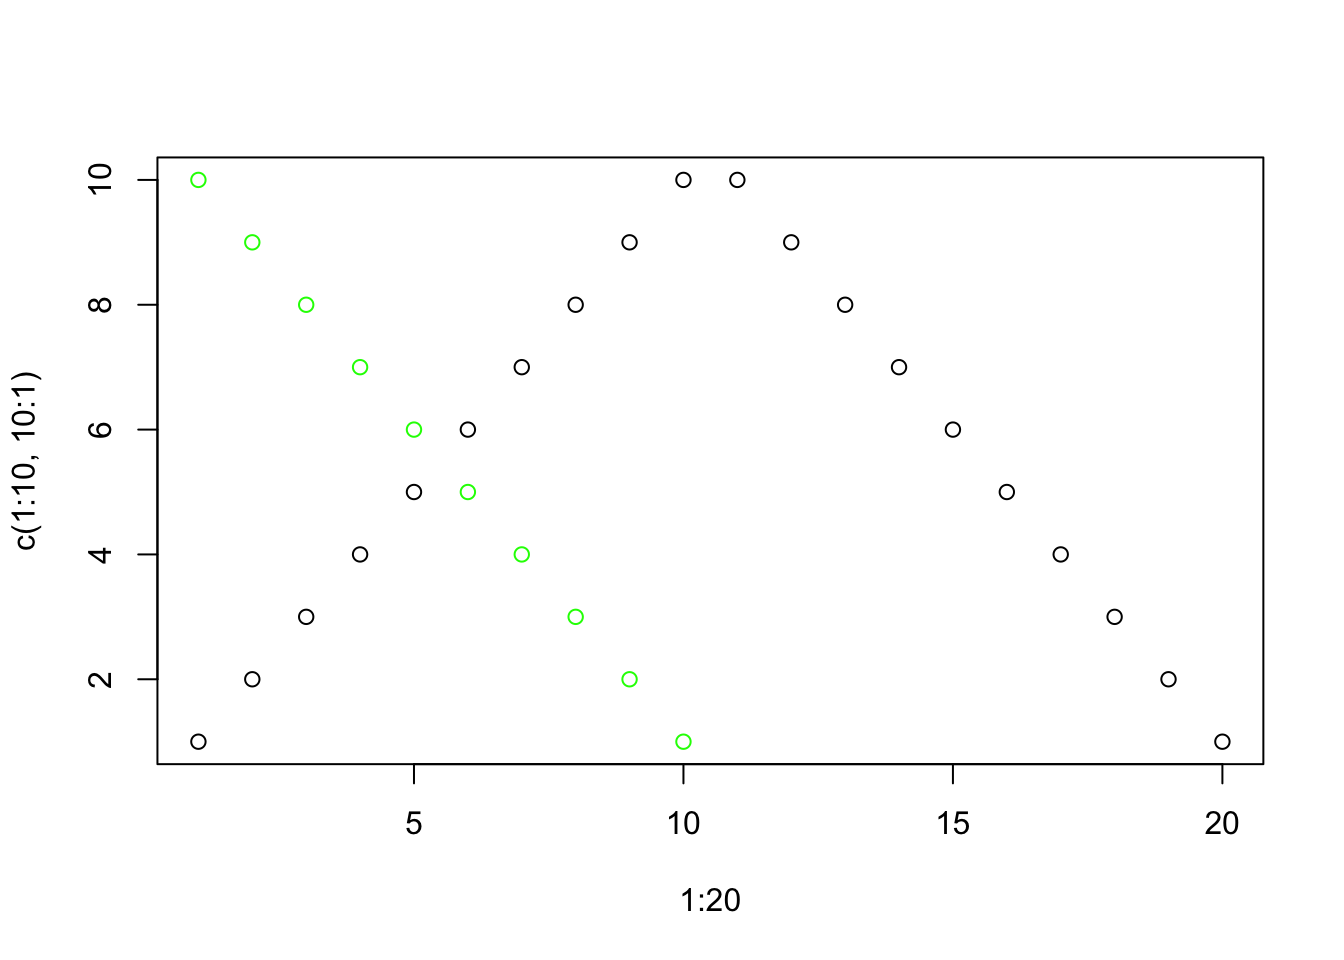
\includegraphics{Intensive-Stats-R_files/figure-latex/unnamed-chunk-1-1.pdf}
To draw connected line segments instead of points, use
\texttt{type="l"}; to add line segments to an existing plot, use
\texttt{lines} (for a pair of vectors) or \texttt{curve} (for a
function).

\begin{Shaded}
\begin{Highlighting}[]
\KeywordTok{plot}\NormalTok{(}\DecValTok{1}\OperatorTok{:}\DecValTok{20}\NormalTok{, }\KeywordTok{c}\NormalTok{(}\DecValTok{1}\OperatorTok{:}\DecValTok{10}\NormalTok{, }\DecValTok{10}\OperatorTok{:}\DecValTok{1}\NormalTok{), }\DataTypeTok{type=}\StringTok{"l"}\NormalTok{,}
     \DataTypeTok{main=}\StringTok{"Demonstrating lines"}\NormalTok{)}
\KeywordTok{lines}\NormalTok{(}\DecValTok{1}\OperatorTok{:}\DecValTok{10}\NormalTok{, }\DecValTok{10}\OperatorTok{:}\DecValTok{1}\NormalTok{, }\DataTypeTok{col=}\StringTok{"green"}\NormalTok{, }\DataTypeTok{lwd=}\DecValTok{3}\NormalTok{) }\CommentTok{# lwd sets line width}
\KeywordTok{curve}\NormalTok{(}\KeywordTok{log}\NormalTok{(x), }\DataTypeTok{col=}\StringTok{"blue"}\NormalTok{, }\DataTypeTok{add=}\OtherTok{TRUE}\NormalTok{)}
\end{Highlighting}
\end{Shaded}

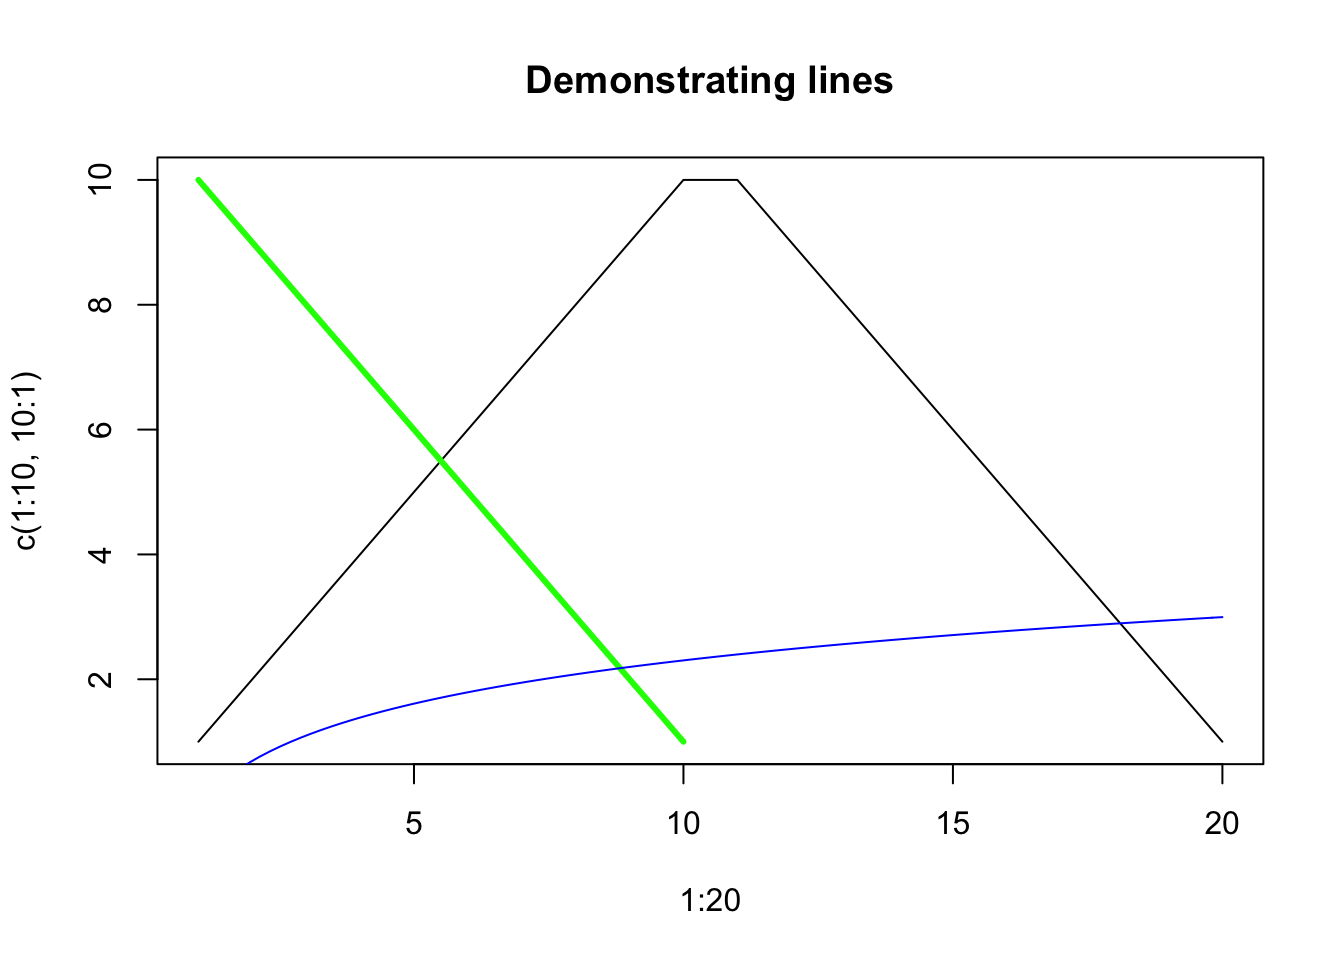
\includegraphics{Intensive-Stats-R_files/figure-latex/unnamed-chunk-2-1.pdf}

The distribution of a numerical vector can be checked for normality
using a \emph{Normal quantile plot} which is a scatterplot of the
vector's ordered values paired with idealized ordered values of a truly
Normal sample. The R command is \texttt{qqnorm}; for example:

\begin{Shaded}
\begin{Highlighting}[]
\NormalTok{y <-}\StringTok{ }\NormalTok{MASS}\OperatorTok{::}\NormalTok{Traffic}\OperatorTok{$}\NormalTok{y}
\KeywordTok{par}\NormalTok{(}\DataTypeTok{mfrow=}\KeywordTok{c}\NormalTok{(}\DecValTok{3}\NormalTok{, }\DecValTok{2}\NormalTok{))}
\KeywordTok{qqnorm}\NormalTok{(y, }\DataTypeTok{main=}\StringTok{"Traffic"}\NormalTok{)}
\ControlFlowTok{for}\NormalTok{(i }\ControlFlowTok{in} \DecValTok{1}\OperatorTok{:}\DecValTok{5}\NormalTok{) \{}
  \KeywordTok{qqnorm}\NormalTok{(}\KeywordTok{rnorm}\NormalTok{(}\KeywordTok{length}\NormalTok{(y)), }\DataTypeTok{main=}\KeywordTok{paste}\NormalTok{(}\StringTok{"Normal sample"}\NormalTok{, i))}
\NormalTok{\}}
\end{Highlighting}
\end{Shaded}

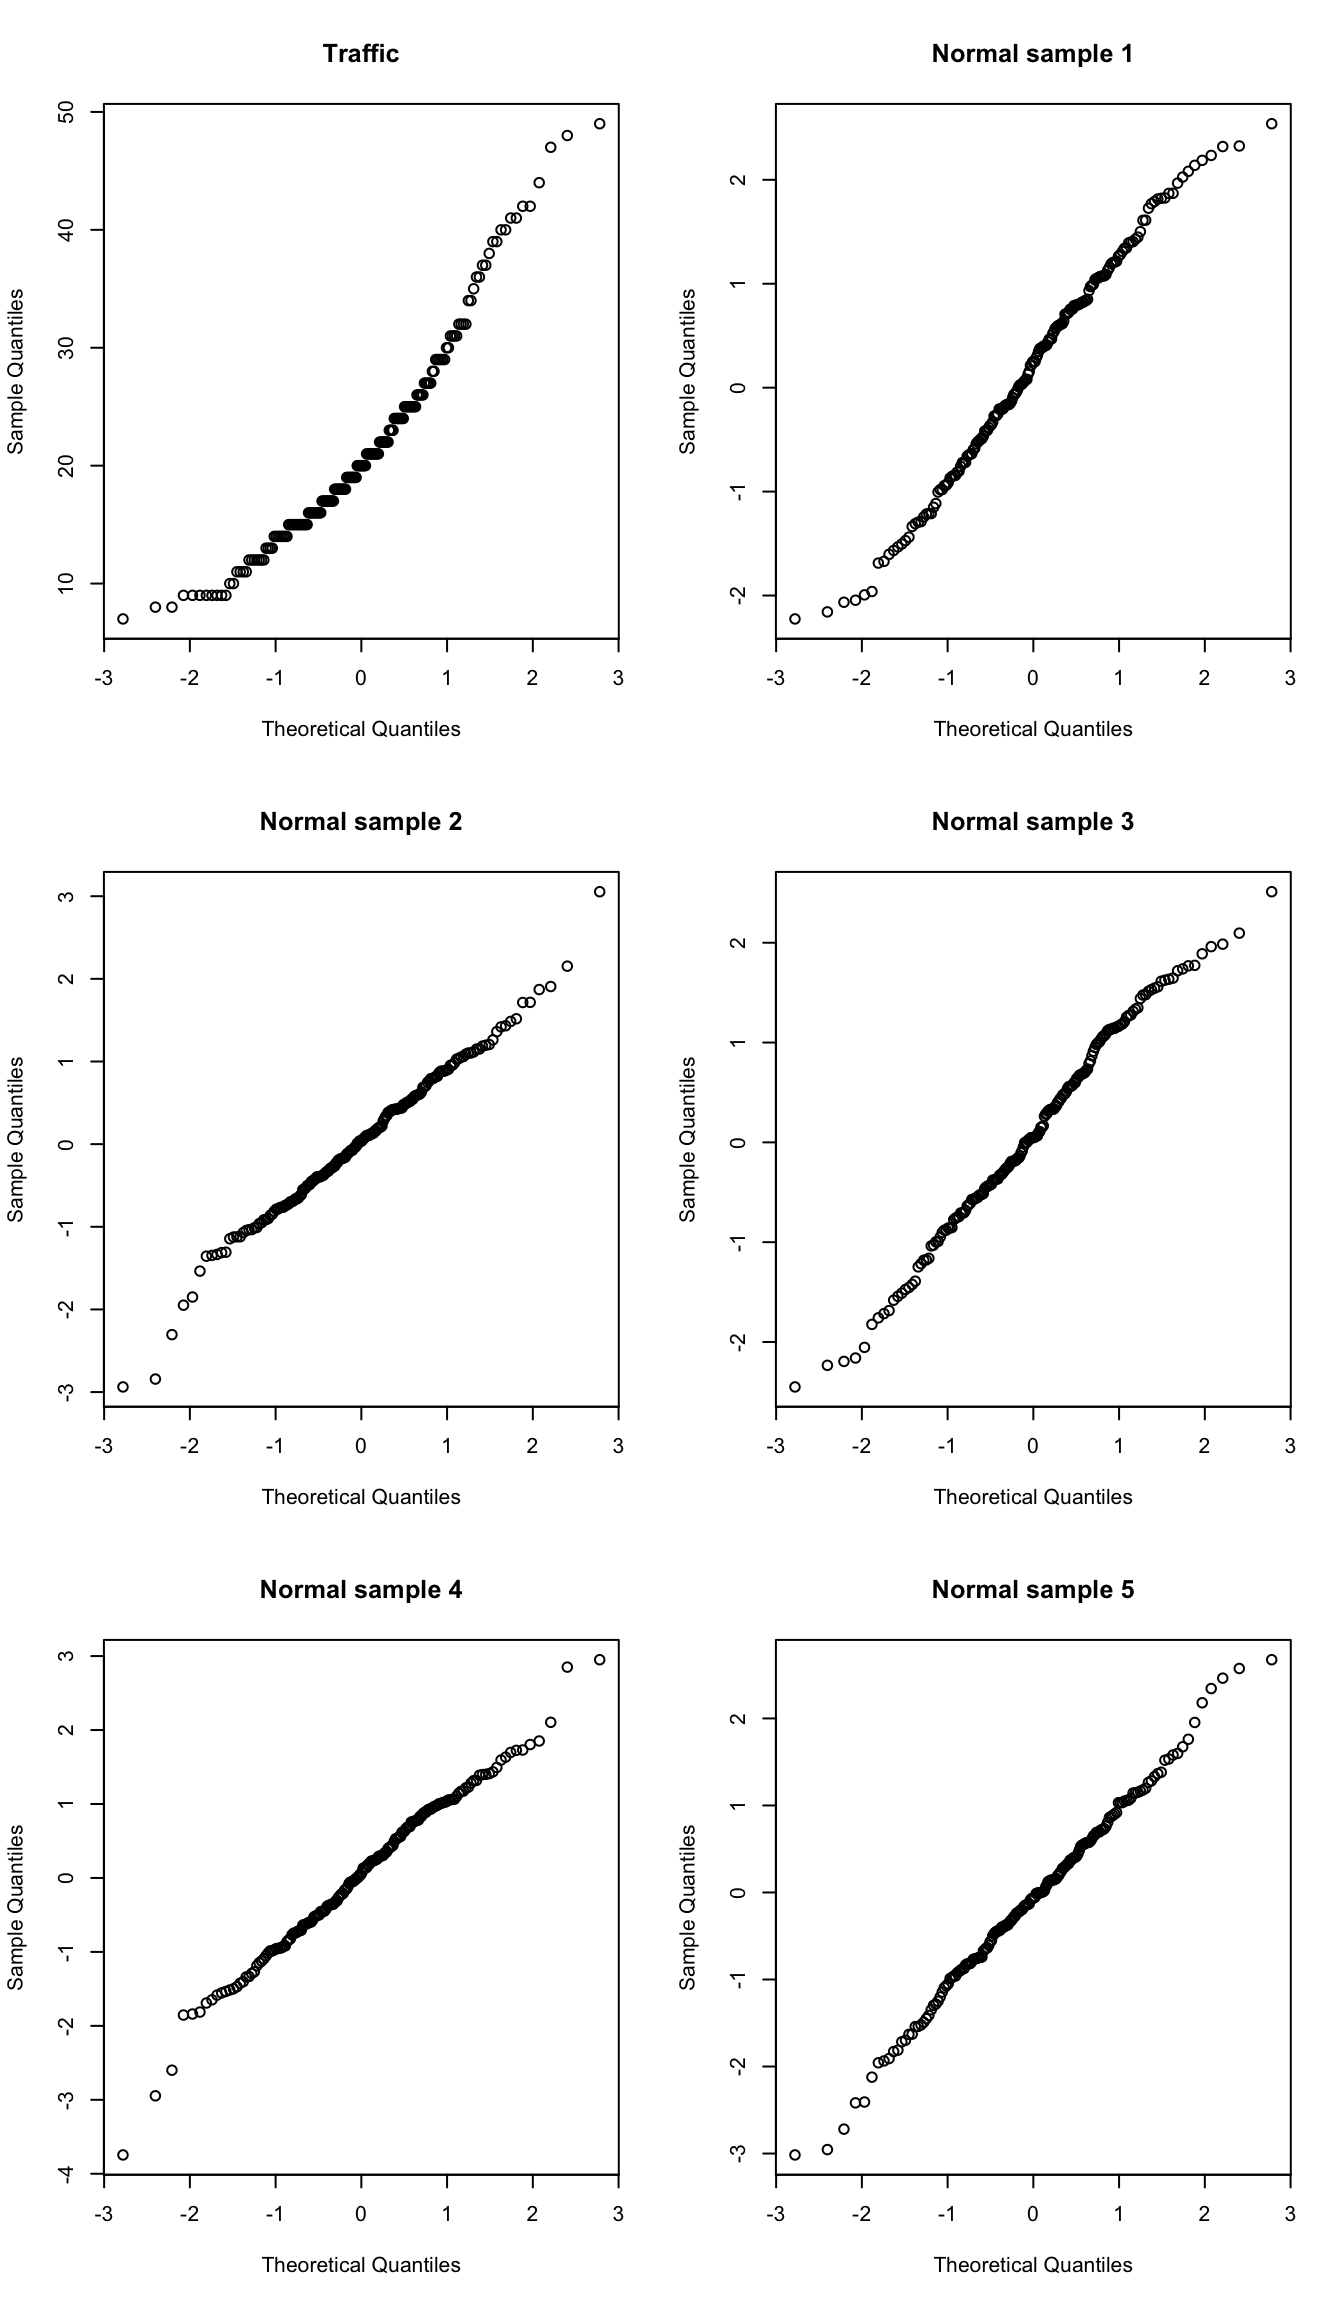
\includegraphics{Intensive-Stats-R_files/figure-latex/unnamed-chunk-3-1.pdf}

\begin{Shaded}
\begin{Highlighting}[]
\KeywordTok{par}\NormalTok{(}\DataTypeTok{mfrow=}\KeywordTok{c}\NormalTok{(}\DecValTok{1}\NormalTok{, }\DecValTok{1}\NormalTok{))}
\end{Highlighting}
\end{Shaded}

The \texttt{par(mfrow=c(3,\ 2))} command told the interpreter to place
the next six plots together in a 3 by 2 grid.

\hypertarget{markdown}{%
\chapter{Markdown}\label{markdown}}

A language called \emph{Markdown} is commonly used to indicate simple
structure and formatting within a plain text file without cluttering it.
The text is processed by a parsing program which turns it into a
structured and formatted document. As a very simple example, ``this
*Markdown* text'' gets displayed as ``this \emph{Markdown} text''; text
that lies between asterisks gets italicized. Markdown also makes it easy
to make bold text, create links, create tables, insert images, write
LaTeX math, and the list goes on. See RStudio's
\href{https://rmarkdown.rstudio.com/authoring_pandoc_markdown.html}{guide}
for more.

We will use a language called R Markdown to write nice polished
documents that fluidly incorporate R code and plots. From the RStudio
menu, select File \textgreater{} New File \textgreater{} R Markdown.
Make the title ``Nice Example'' and click OK. RStudio opens a simple
example R Markdown (Rmd) file. Go to File \textgreater{} Knit Document
(and make note of the hotkey); RStudio will prompt you to save the file,
then it will display the processed example document as a webpage. In the
file editor, change the first sentence under ``\#\# R Markdown'' to
``This is my *first* R Markdown document.'' Then press the Knit Document
hotkey again to see your change implemented.

R Markdown does ordinary markdown parsing, but it does a bit of extra
processing first. It looks for R code to run; notice what happens with
\texttt{summary(cars)} and \texttt{plot(pressure)} from the Rmd file. R
Markdown displays your R code neatly, along with the interpreter's
output and plots.

\begin{center}\rule{0.5\linewidth}{\linethickness}\end{center}

\textbf{Exercise:} Change ``\{r pressure, echo=FALSE\}'' to ``\{r\}''
and knit the document again. What do you think ``pressure'' and
``echo=FALSE'' were doing?

\begin{center}\rule{0.5\linewidth}{\linethickness}\end{center}

\textbf{Exercise:} At the top of the Rmd file, change ``html\_document''
to ``pdf\_document'' then Knit Document again.

\begin{center}\rule{0.5\linewidth}{\linethickness}\end{center}

The package \href{https://yihui.name/knitr/options/}{knitr} is used for
specifying how you want to handle each
\href{https://rmarkdown.rstudio.com/lesson-3.html}{code chunk}, for
instance, if you want to change the size of a plot.

Glance over this
\href{http://www.stat.cmu.edu/~cshalizi/rmarkdown/}{beginner's guide} to
get an idea of what else R Markdown can do.

\hypertarget{probability}{%
\chapter{Probability}\label{probability}}

\hypertarget{sampling-from-a-vector}{%
\section{Sampling from a vector}\label{sampling-from-a-vector}}

The \texttt{sample} command draws a specified number of entries from a
vector. If you want to randomly pick three (numbered) students from a
class of ten, you can run \texttt{sample(1:10,\ 3)}.

Sometimes you want to draw \emph{with replacement}, meaning that each
pick ignores what has happened previously; after each draw, you
\emph{replace} your pick before drawing again. For instance, if you want
to randomly assign twenty tasks to four employees, you could run
\texttt{sample(1:4,\ 20,\ replace=TRUE)}. If you want employee number 1
to have twice as large of a probability as the other employees of being
assigned each task, you'll need to use the \texttt{prob} parameter:
\texttt{sample(1:4,\ 20,\ replace=TRUE,\ prob=c(2,\ 1,\ 1,\ 1)}.

\hypertarget{four-basic-functions-for-common-distributions}{%
\section{Four basic functions for common
distributions}\label{four-basic-functions-for-common-distributions}}

For several families of distributions, the R language has four built-in
functions corresponding to:

\begin{itemize}
\tightlist
\item
  Density (pdf for continuous distributions, pmf for discrete
  distributions)
\item
  Probability less than or equal (cdf)
\item
  Quantile (inverse cdf)
\item
  Random sample
\end{itemize}

The function names follow the pattern ``d,'' ``p,'' ``q,'' or ``r''
followed by an abbreviation for the family of distributions. For
example, the probability of getting four heads out of ten flips of a
coin with heads-probability .25 is calculated by the R command
\texttt{dbinom(4,\ 10,\ .25)}. The probability of four or fewer heads is
\texttt{pbinom(4,\ 10,\ .25)}. Next, \texttt{qbinom(.95,\ 10,\ .25)}
tells you the smallest number of heads for which there is no more than
.05 probability of exceeding. Finally, \texttt{rbinom(100,\ 10,\ .25)}
simulates one hundred experiments of the twenty coin flips and tells you
how many heads it got in each trial.

For Normal distributions, the abbreviation is ``norm.'' If no additional
parameters are specified, it assumes you want mean zero and standard
deviation one. Otherwise use the second and third parameters (named
``mean'' and ``sd'').

Binomial distributions are discrete whereas Normal distributions are
continuous. The four functions work in both cases.

\begin{Shaded}
\begin{Highlighting}[]
\KeywordTok{plot}\NormalTok{(}\DecValTok{0}\OperatorTok{:}\DecValTok{10}\NormalTok{, }\KeywordTok{dbinom}\NormalTok{(}\DecValTok{0}\OperatorTok{:}\DecValTok{10}\NormalTok{, }\DecValTok{10}\NormalTok{, }\FloatTok{.25}\NormalTok{))}
\KeywordTok{curve}\NormalTok{(}\KeywordTok{dnorm}\NormalTok{(x, }\DataTypeTok{mean=}\DecValTok{10}\OperatorTok{*}\NormalTok{.}\DecValTok{25}\NormalTok{, }\DataTypeTok{sd=}\KeywordTok{sqrt}\NormalTok{(}\DecValTok{10}\OperatorTok{*}\NormalTok{.}\DecValTok{25}\OperatorTok{*}\NormalTok{.}\DecValTok{75}\NormalTok{)), }\DataTypeTok{from=}\DecValTok{0}\NormalTok{, }\DataTypeTok{to=}\DecValTok{10}\NormalTok{, }\DataTypeTok{add=}\OtherTok{TRUE}\NormalTok{, }\DataTypeTok{col=}\DecValTok{2}\NormalTok{)}
\end{Highlighting}
\end{Shaded}

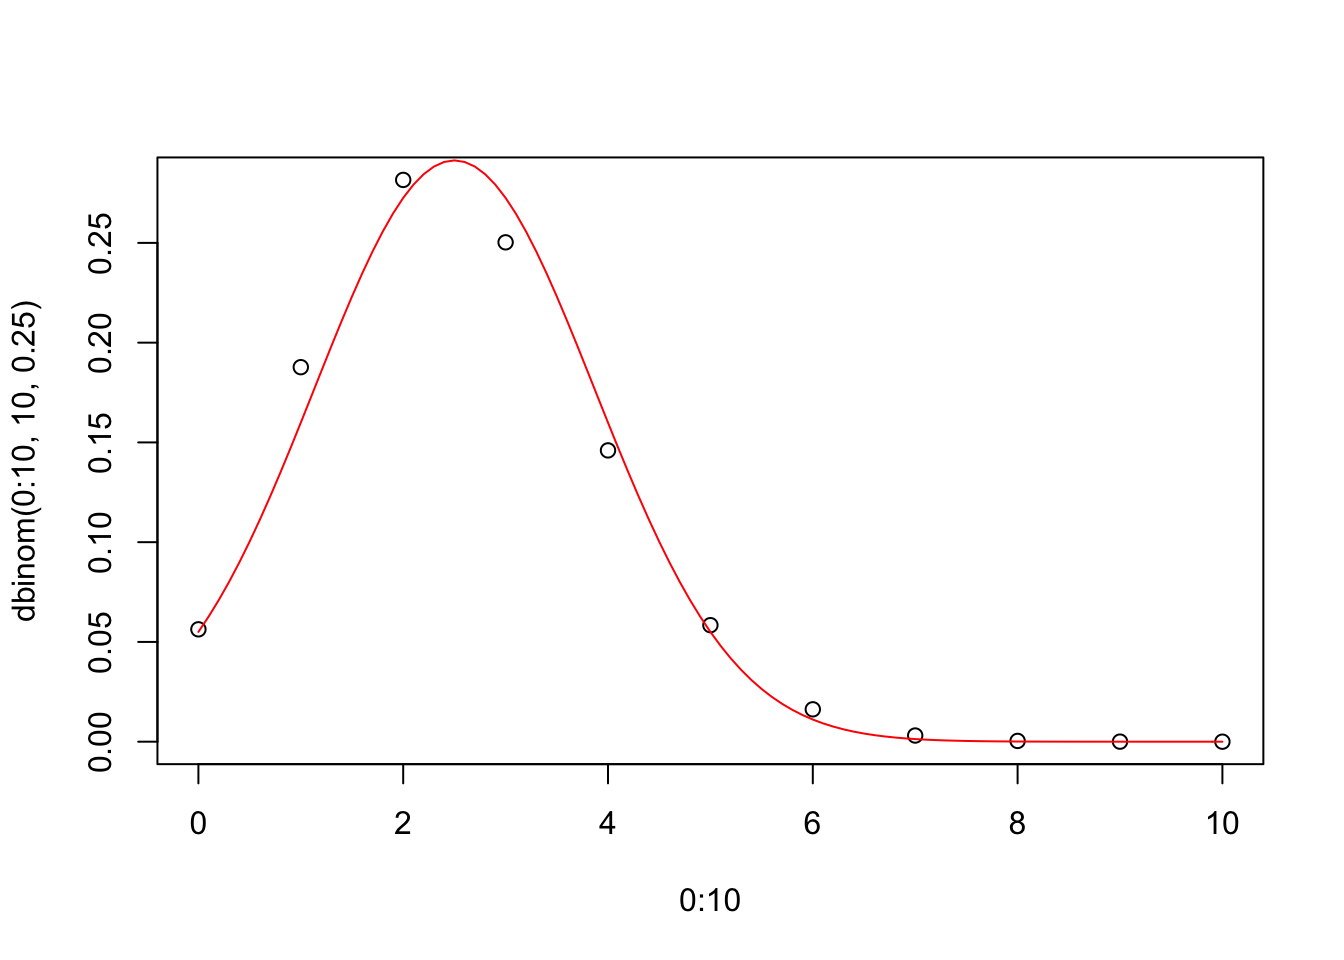
\includegraphics{Intensive-Stats-R_files/figure-latex/unnamed-chunk-4-1.pdf}

Another family built in to R is the uniform distributions, abbreviated
``unif.'' In particular, \texttt{runif(n)} generates \texttt{n}
independent draws from the Uniform(0, 1) distribution.

Before asking the R interpreter to perform a random draw, you might want
to use the \texttt{set.seed} command with any integer as the input. This
sets a ``starting point'' for the random draw so that the exact same
``random'' results can be replicated by the code at a later time or by
another computer.

\begin{Shaded}
\begin{Highlighting}[]
\KeywordTok{runif}\NormalTok{(}\DecValTok{5}\NormalTok{)}
\end{Highlighting}
\end{Shaded}

\begin{verbatim}
## [1] 0.67451841 0.28798486 0.62727115 0.03874901 0.54447534
\end{verbatim}

\begin{Shaded}
\begin{Highlighting}[]
\KeywordTok{set.seed}\NormalTok{(}\DecValTok{1}\NormalTok{)}
\KeywordTok{runif}\NormalTok{(}\DecValTok{5}\NormalTok{)}
\end{Highlighting}
\end{Shaded}

\begin{verbatim}
## [1] 0.2655087 0.3721239 0.5728534 0.9082078 0.2016819
\end{verbatim}

When you run the above code, my first \texttt{runif(5)} output will
differ from yours, but our draws will agree after we've both set the
seed to 1.

\hypertarget{simulation}{%
\section{Simulation}\label{simulation}}

In a room of 100 people, is it likely that you will be able to find a
birthday shared by two people? What about three people? Four? Let's
pretend that leap-years don't exist, that each day of the year is
equally likely to be a person's birthday, and that the people's
birthdays are independent. Now we draw random birthdays accordingly.

\begin{Shaded}
\begin{Highlighting}[]
\NormalTok{n <-}\StringTok{ }\DecValTok{100}
\KeywordTok{set.seed}\NormalTok{(}\DecValTok{4}\NormalTok{)}
\NormalTok{b <-}\StringTok{ }\KeywordTok{sample}\NormalTok{(}\DecValTok{1}\OperatorTok{:}\DecValTok{365}\NormalTok{, n, }\DataTypeTok{replace=}\OtherTok{TRUE}\NormalTok{)}
\NormalTok{b}
\end{Highlighting}
\end{Shaded}

\begin{verbatim}
##   [1] 214   4 108 102 297  96 265 331 347  27 276 105  37 349 152 167 355
##  [18] 214 352 279 261 364 185 179 237 304 176 308 188 194 207  88 321 239
##  [35] 177 355 168 228 142   3 343  89 207  67 331  31 329 326 265 207 142
##  [52] 273 327 296 299 154  65  64 326 272 205  27 312 334  83 230  26 188
##  [69] 294 355 126 231 150 127 302 252 118 162  96  49 333 259 209 335 330
##  [86]  22  17 361  76 340  71  47 197 100 130  31 280 163  14 256
\end{verbatim}

\begin{Shaded}
\begin{Highlighting}[]
\KeywordTok{table}\NormalTok{(b)}
\end{Highlighting}
\end{Shaded}

\begin{verbatim}
## b
##   3   4  14  17  22  26  27  31  37  47  49  64  65  67  71  76  83  88 
##   1   1   1   1   1   1   2   2   1   1   1   1   1   1   1   1   1   1 
##  89  96 100 102 105 108 118 126 127 130 142 150 152 154 162 163 167 168 
##   1   2   1   1   1   1   1   1   1   1   2   1   1   1   1   1   1   1 
## 176 177 179 185 188 194 197 205 207 209 214 228 230 231 237 239 252 256 
##   1   1   1   1   2   1   1   1   3   1   2   1   1   1   1   1   1   1 
## 259 261 265 272 273 276 279 280 294 296 297 299 302 304 308 312 321 326 
##   1   1   2   1   1   1   1   1   1   1   1   1   1   1   1   1   1   2 
## 327 329 330 331 333 334 335 340 343 347 349 352 355 361 364 
##   1   1   1   2   1   1   1   1   1   1   1   1   3   1   1
\end{verbatim}

\begin{Shaded}
\begin{Highlighting}[]
\KeywordTok{max}\NormalTok{(}\KeywordTok{table}\NormalTok{(b))}
\end{Highlighting}
\end{Shaded}

\begin{verbatim}
## [1] 3
\end{verbatim}

The \texttt{table} command scans through a vector and counts the number
of occurrences of each value. The \texttt{max} tells us that there is at
least one birthday shared by three people but no birthdays are shared by
four or more.

But this is a single run of the experiment. To get a better idea of the
range of possible outcomes and how probable they are, we want to run the
experiment a large number of times.

\begin{Shaded}
\begin{Highlighting}[]
\NormalTok{nsim <-}\StringTok{ }\DecValTok{10000}
\NormalTok{results <-}\StringTok{ }\KeywordTok{rep}\NormalTok{(}\OtherTok{NA}\NormalTok{, nsim)}
\ControlFlowTok{for}\NormalTok{(i }\ControlFlowTok{in} \DecValTok{1}\OperatorTok{:}\NormalTok{nsim) \{}
\NormalTok{  b <-}\StringTok{ }\KeywordTok{sample}\NormalTok{(}\DecValTok{1}\OperatorTok{:}\DecValTok{365}\NormalTok{, n, }\DataTypeTok{replace=}\OtherTok{TRUE}\NormalTok{)}
\NormalTok{  results[i] <-}\StringTok{ }\KeywordTok{max}\NormalTok{(}\KeywordTok{table}\NormalTok{(b))}
\NormalTok{\}}
\KeywordTok{table}\NormalTok{(results)}\OperatorTok{/}\NormalTok{nsim}
\end{Highlighting}
\end{Shaded}

\begin{verbatim}
## results
##      2      3      4      5      6 
## 0.3598 0.5786 0.0586 0.0029 0.0001
\end{verbatim}

\begin{center}\rule{0.5\linewidth}{\linethickness}\end{center}

\textbf{Exercise:} The following simulation code runs fine, but it
doesn't perform a valid simulation. Identify the TWO flaws and fix them.

\begin{verbatim}
n <- 100
nsim <- 10000
results <- rep(NA, nsim)
for(i in 1:nsim) {
  set.seed(3)
  results <- max(rnorm(n))
}
\end{verbatim}

Run your fixed version of the simulation and plot a \texttt{truehist} of
the results.

\begin{center}\rule{0.5\linewidth}{\linethickness}\end{center}

\hypertarget{statistics}{%
\chapter{Statistics}\label{statistics}}

\hypertarget{binomial-statistics}{%
\section{Binomial statistics}\label{binomial-statistics}}

Suppose a casino game involves flipping a coin that they claim is fair,
i.e.~that heads and tails are equally probable. The casino wins the bet
when which tails is flipped, while you win if it's heads. You play the
game 1000 times and observe only 429 heads. Should you doubt the
casino's claim that the coin is fair? We could use \texttt{pbinom} to
calculate the exact significance probability, but let's instead try
\texttt{prop.test} which uses the Normal approximation with a continuity
correction to give a significance probability and confidence interval.
(Add the parameter \texttt{correct=F} to suppress the continuity
correction.)

\begin{Shaded}
\begin{Highlighting}[]
\KeywordTok{prop.test}\NormalTok{(}\DecValTok{429}\NormalTok{, }\DecValTok{1000}\NormalTok{, }\DataTypeTok{alternative=}\StringTok{"less"}\NormalTok{)}
\end{Highlighting}
\end{Shaded}

\begin{verbatim}
## 
##  1-sample proportions test with continuity correction
## 
## data:  429 out of 1000, null probability 0.5
## X-squared = 19.881, df = 1, p-value = 4.121e-06
## alternative hypothesis: true p is less than 0.5
## 95 percent confidence interval:
##  0.0000000 0.4554038
## sample estimates:
##     p 
## 0.429
\end{verbatim}

If the coin really is fair, there's less than a one in ten thousand
chance of an outcome at least this small. If the casino had instead
claimed that the coin had heads probability of .48, you could test that
by adding the parameter \texttt{p=.48} to the function call.

To test the other extreme with \texttt{prop.test}, use
\texttt{alternative="greater"}; a two-sided test is used by default if
you do not specify a value for \texttt{alternative}.

There are a variety of opinions about how to calculate confidence
intervals for a Binomial success probability. A number of methods are
provided by \texttt{binom.confint} in the \texttt{binom} package. (Do
\texttt{install.packages("binom")} before running the code below.)

\begin{Shaded}
\begin{Highlighting}[]
\KeywordTok{library}\NormalTok{(binom)}
\KeywordTok{binom.confint}\NormalTok{(}\DecValTok{429}\NormalTok{, }\DecValTok{1000}\NormalTok{, }\DataTypeTok{conf.level=}\FloatTok{0.95}\NormalTok{, }\DataTypeTok{methods=}\StringTok{"all"}\NormalTok{)}
\end{Highlighting}
\end{Shaded}

\begin{verbatim}
##           method   x    n      mean     lower     upper
## 1  agresti-coull 429 1000 0.4290000 0.3986523 0.4598911
## 2     asymptotic 429 1000 0.4290000 0.3983243 0.4596757
## 3          bayes 429 1000 0.4290709 0.3984722 0.4597491
## 4        cloglog 429 1000 0.4290000 0.3981561 0.4594475
## 5          exact 429 1000 0.4290000 0.3980720 0.4603472
## 6          logit 429 1000 0.4290000 0.3986339 0.4599102
## 7         probit 429 1000 0.4290000 0.3985686 0.4598596
## 8        profile 429 1000 0.4290000 0.3985352 0.4598282
## 9            lrt 429 1000 0.4290000 0.3985450 0.4598228
## 10     prop.test 429 1000 0.4290000 0.3981599 0.4603924
## 11        wilson 429 1000 0.4290000 0.3986535 0.4598899
\end{verbatim}

\begin{center}\rule{0.5\linewidth}{\linethickness}\end{center}

\textbf{Exercise:} Run a two-sided \texttt{prop.test} to see which of
the \texttt{binom.confint} methods it agrees with.

\begin{center}\rule{0.5\linewidth}{\linethickness}\end{center}

\hypertarget{more-to-come}{%
\section{More to come}\label{more-to-come}}

\bibliography{book.bib}


\end{document}
